\begin{samepage}
\subsection{Entity-Relationship Schema}
\begin{figure}
\centering
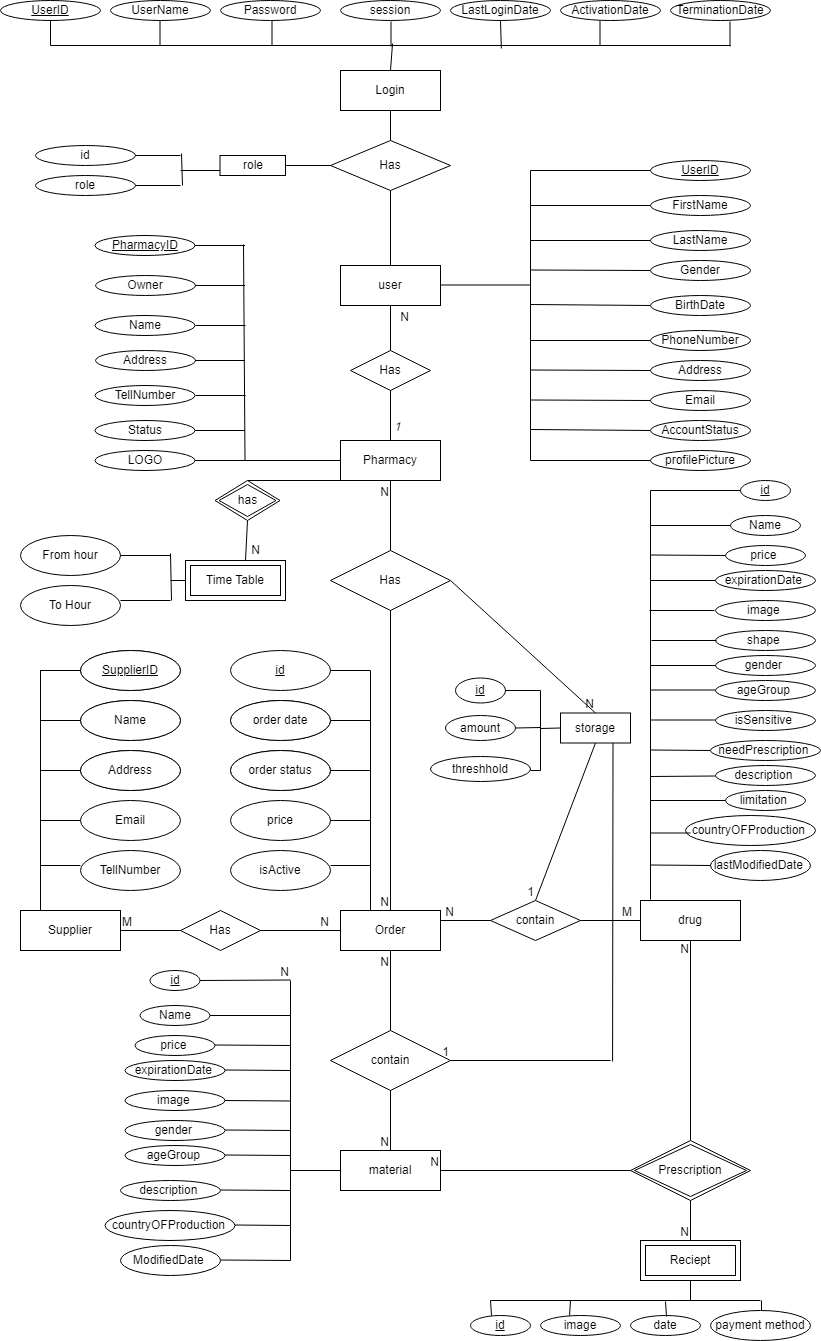
\includegraphics[width=0.72\textwidth]{sections/DLL/ED.png}
\caption{Entity-Relationship Schema}
\label{fig:ER}
\end{figure}
\end{samepage}
%Describe here your ER schema
The Entity-Relationship schema of this project (Figure~\ref{fig:ER}) contains 11 main entities:
\begin{itemize}
\item \emph{pharmacy}: An entity named Pharmacy  has several attributes, including an ID, a name, an address, a telephone number, a list of opening times, a logo image, a list of stored items, and a list of staff members.
\item \emph{TimeTable}: this entity is a system that represents the opening hours of a pharmacy. It has attributes such as an id, $from\_hour$, and $to\_hour$ strings which represent the start and end times for a given opening period. 
 \item \emph{User}: The \emph{User} is an entity in a system that represents a user. It has various attributes such as name, last name, gender, birth date, phone number, address, role, email, account status, profile picture, and pharmacy.
 \item \emph{role}: The \emph{Role} is an entity that represents a database table with an ID and a unique role name.
 \item \emph{login}: The entity contains numerous attributes, such as an automatically generated ID, a username, a password, and a session flag. Additionally, it holds information regarding the user's last login time, activation date, termination date, and a reference to another User object. 
  \item \emph{Supplier}: it is an entity in a system that represents a supplier. It has various attributes such as an id, name, address, email, and telephone number. It also has two lists of drugs and materials that the supplier provides.
  \item \emph{order}: The ordering entity  has several attributes, including an ID, an order date, lists of drugs and materials, an order status, a price, and an active status.
  \item \emph{Storage}: This is an entity in a system that represents the number of drugs and materials available at a pharmacy. It has attributes such as an id, amount (the quantity of the drug or material stored), and threshold (the minimum amount of a drug or material that must be kept in stock).
  \item \emph{drug}: The Drug is an entity that represents a drug in a database. It contains 16 attributes, including id, name, supplier, expirationDate, image, shape, gender (the gender specification of the drug), ageGroup (the age group that the drug is intended for), isSensitive (a boolean value indicating if the drug is sensitive), needPrescription (a boolean value indicating if the drug requires a prescription), description, limitation (the number of drugs that a patient can purchase), price, countryOFProduction (the country of production for the drug), lastModifiedDate(the date and time the drug was last modified) 
  \item \emph{material}: Material entity is similar to drug entity. It has an ID, a name, a supplier, a country of production, an expiration date, an image, a gender, a price, an age group, a last modified date, and a description. 
  \item  \emph{reciept}: The entity has several attributes, including an ID, lists of drugs and materials, an image of the receipt, a date, and a payment method. 
\end{itemize}


\
\\
\
\\
\
\\
\\
\
